% In this chapter, we analyze the sixth and last experiment group, that is, the proof of concept of Vertical Blockchain-based Federated Learning. 
The goal of this chapter is to prove that, even though there is a lack of Blockchain-based Federated Learning systems applied to vertically partitioned FL systems, it is possible to do so.

This experiment was performed with two different number of clients: 2 and 4, with a dual-headed, and four-headed Split-CNN model, respectively. In addition, most Vertical Federated Learning models from the literature were applied to 2 clients. Therefore, it is interesting to see that it is possible to easily apply the model to more clients.

\section{Execution Time, Transaction Cost, and Transaction Latency}

The execution time and transaction metrics can be seen in \autoref{tab:metrics_vertical}. It is observable that the more the clients, the longer a round takes to be completed. As such the entire learning process takes longer. This is a conclusion that was taken in a previous chapters, too.

Regarding the transaction latency and cost, we can see that both are similar to what has been seen in previous chapters. Since the number of clients is low, we did not expect to have significant differences in either of them.

\begin{table}[!ht]
\begin{tabular}{c|c|c} \hline \hline
                                & 2             & 4             \\ \hline \hline
E2E Time (m)                    & 10.97	        & 12.57         \\ \hline
Mean Round Time (s)             & 13.16	        & 15.08         \\ \hline
Mean Transaction Latency (s)    & 1.642	        & 1.546         \\ \hline
Mean Transaction Cost (Gas)     & 141335        & 142638        \\ \hline
\end{tabular}
\caption{Execution Time, Transaction Cost, and Transaction Latency Per Number of Clients}
\label{tab:metrics_vertical}
\end{table}

\section{Accuracy and Convergence}

Regarding accuracy, we can observe smooth convergences, as well as similar high accuracy. Both clients reached an accuracy above $85\%$, only differing in $3\%$. In addition, it is interesting to see that the convergence of the Vertical Federated Learning is much smoother than what we have observed with Horizontal Federated Learning. This is likely explained by the fact that in this setting, all clients participate in each round due to the way the data is structured. In addition, the model is different from a regular CNN, which may lead to different results. However, since both types of data partition solve different types of problems, it is not a fair comparison.

\begin{figure}[!ht]
    \centering
    \centering
    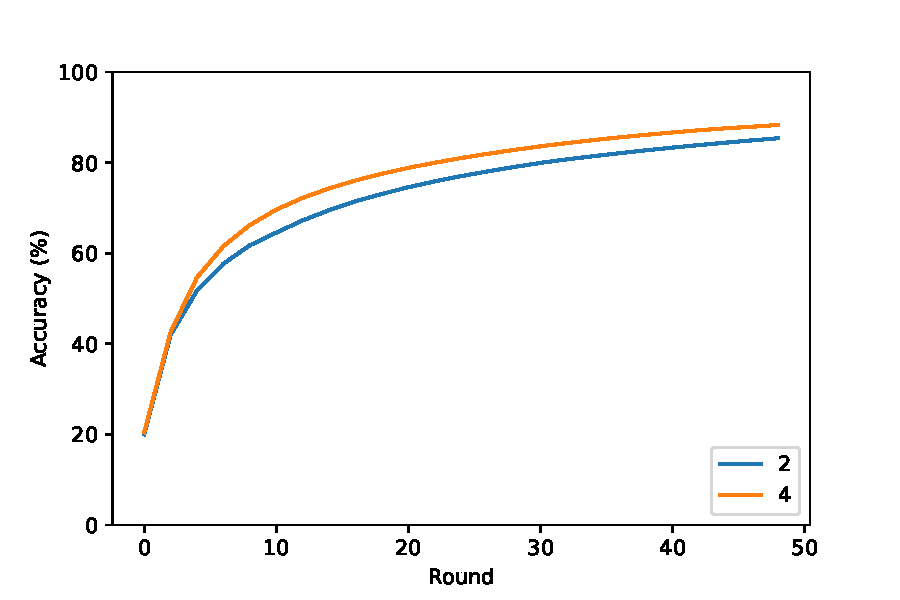
\includegraphics[width=0.7\textwidth]{graphics/vertical/accuracy.pdf}
    \caption{Accuracy Per Number of Clients}
    \label{fig:accuracy_vertical}
\end{figure}

\section{Communication Costs}

The communication costs represented in \autoref{fig:net_vertical} are also within the expected values.

On the clients, we can observe that there is no major difference of traffic when the number of clients increases. This can be explained by the fact that, by using a Split-CNN, each client is only required to upload their own intermediate results and download the gradient updates, which have fixed sizes.

On the servers, the costs are higher with more clients. Since the Split-CNN model has more heads with more clients, the servers are required to download more intermediate results, as well as upload more gradient updates. Therefore, it would be expected that the traffic would double with the double of clients.

On the blockchain, the difference of amount of clients is not significant to make a significant difference on traffic.

\begin{figure}[!ht]
    \centering
    \centering
    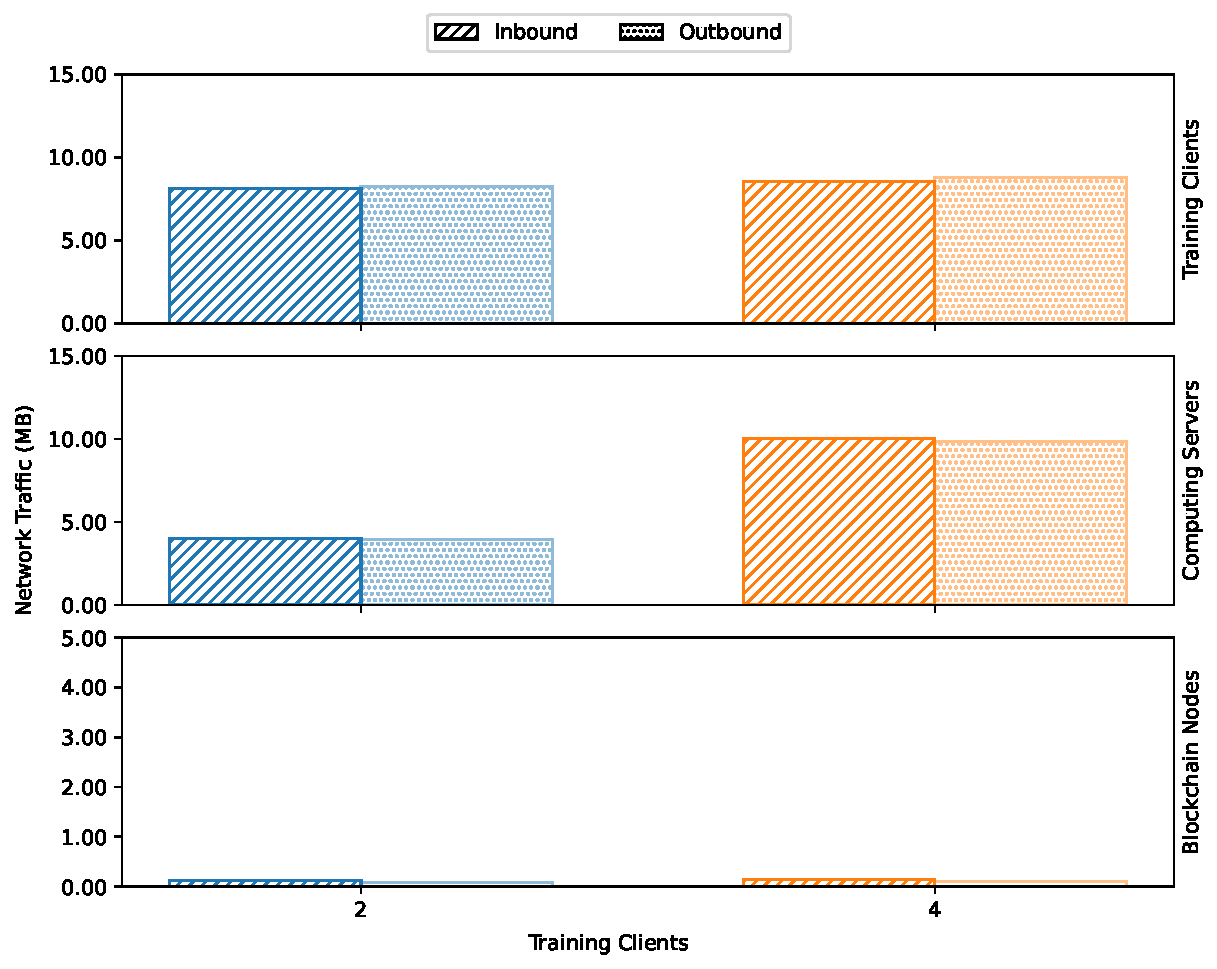
\includegraphics[width=0.8\textwidth]{graphics/vertical/net.pdf}
    \caption{Network Traffic Per Round Per Number of Clients}
    \label{fig:net_vertical}
\end{figure}

\section{Computation Costs}

Computation costs, namely RAM usage and CPU usage, are depicted in \autoref{fig:ram_vertical} and \autoref{fig:cpu_vertical}, respectively. As expected, with higher amounts of clients there is a slightly higher RAM consumption on both the server and blockchain processes, caused by more data being stored in-memory, as well as more messages being carried over the blockchain. However, we see the opposite happening with the clients. This is explained by the fact that the dual-headed CNN contains an additional convolutional layer compared to the four-headed CNN, which leads to more RAM usage during training. Regarding CPU usage, we see similar results as to the RAM usage, which are explained by the same reasons.

\begin{figure}[!ht]
    \centering
    \centering
    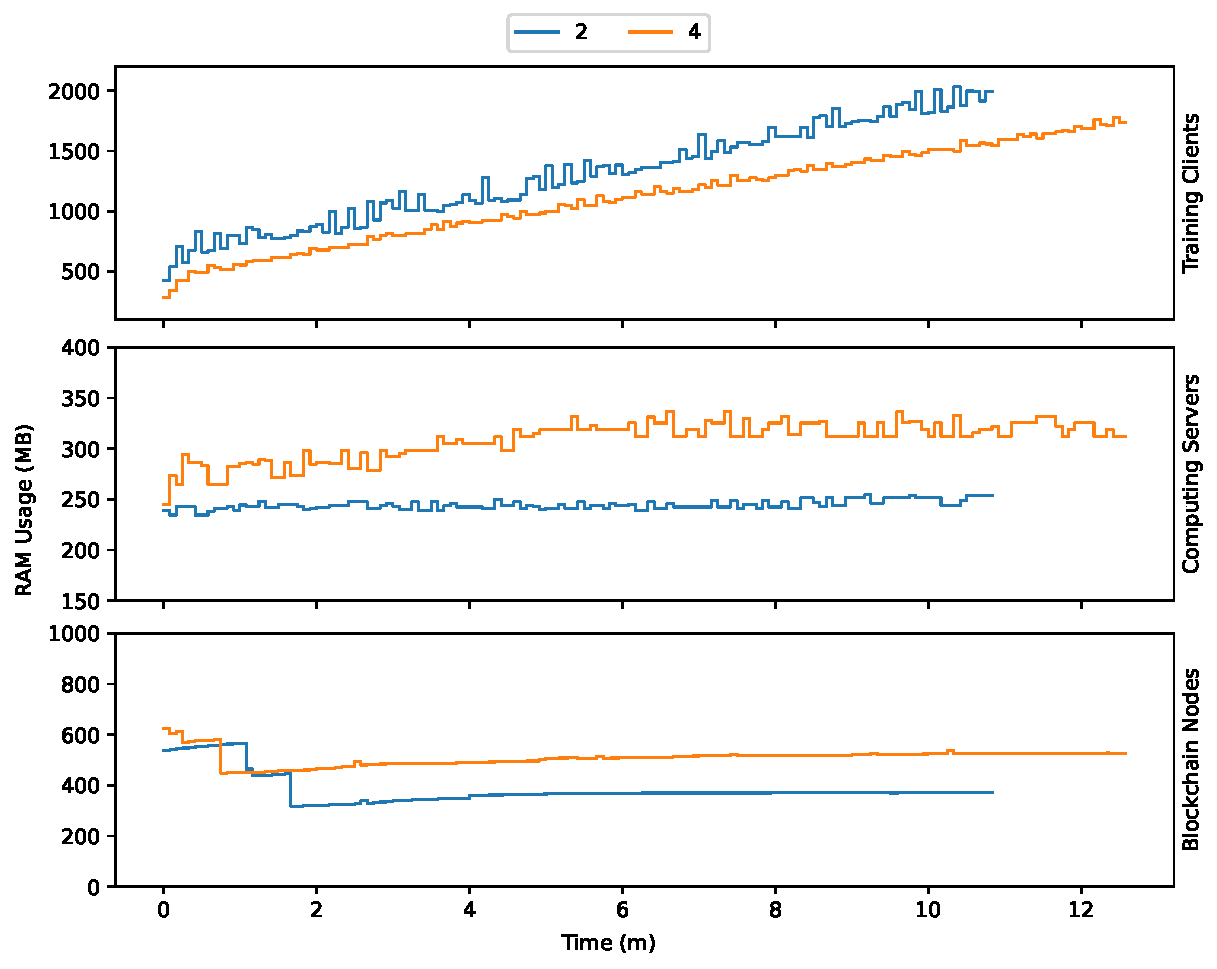
\includegraphics[width=0.8\textwidth]{graphics/vertical/ram.pdf}
    \caption{RAM Usage Per Number of Clients}
    \label{fig:ram_vertical}
\end{figure}

\begin{figure}[!ht]
    \centering
    \centering
    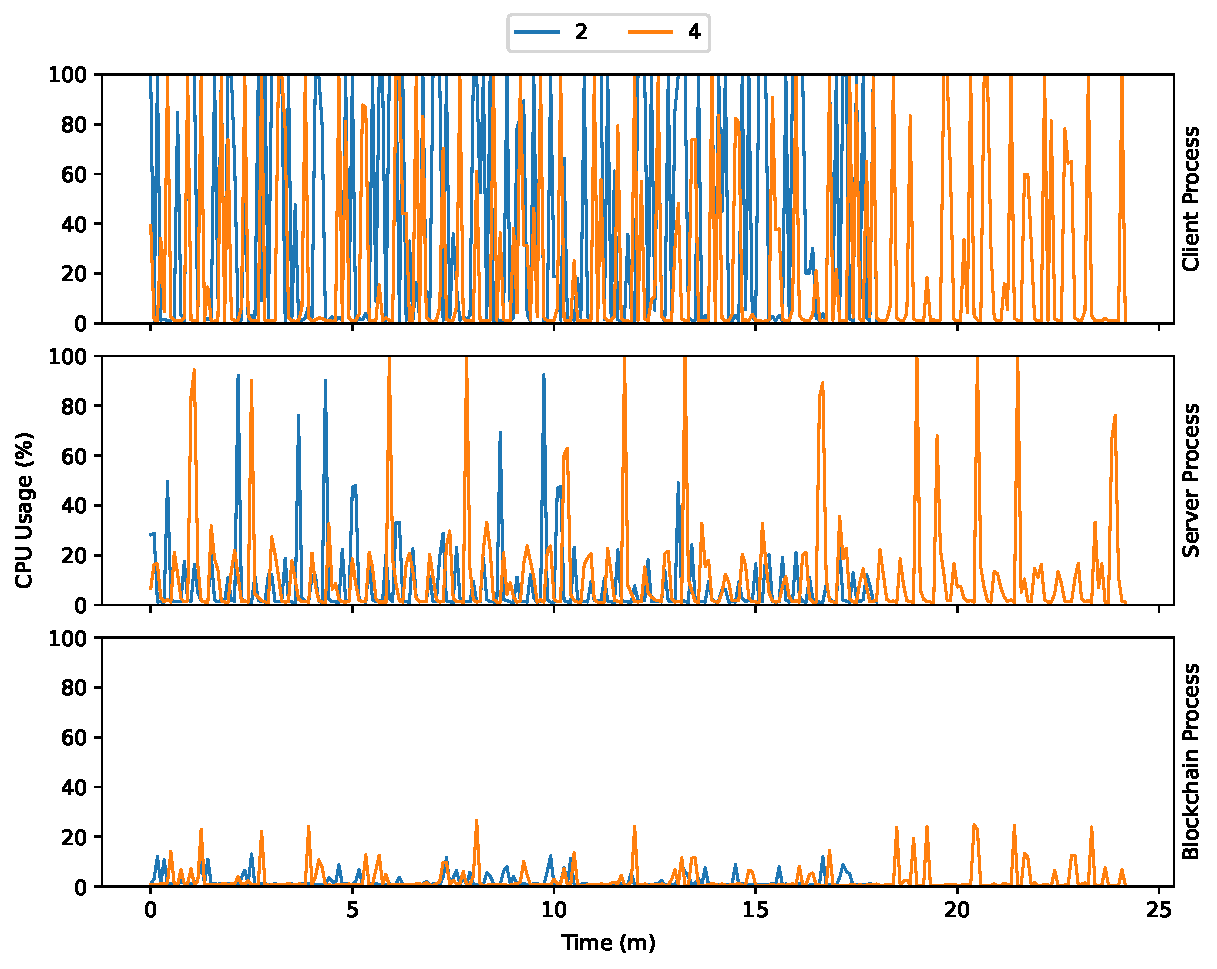
\includegraphics[width=0.8\textwidth]{graphics/vertical/cpu.pdf}
    \caption{CPU Usage Per Number of Clients}
    \label{fig:cpu_vertical}
\end{figure}

\section{Conclusions and Improvements}

From this experiment, we can conclude that it is possible to apply a Blockchain-based Federated Learning system to vertically partitioned data. In future work, it would be interesting to investigate how to apply other models. In addition, it would be interesting to see how other, larger data sets, could be applied with larger amounts of clients. Using MNIST, this experiment is limited because of the extremely small resolution of the images. Therefore, it is not feasible to separate many features. Finally, it would also be worth investigating how privacy mechanisms could be applied to the intermediate model outputs in order to prevent inference attacks.
